\chapter{Privacy Leaks with Digital Photographs}

A digital photograph is nothing more than a collection of
pixels that, when viewed by a human, seems to resemble something that
might be seen with the human eye. Different approaches to digital
photography date back to the 1970s, when large grey-scale photographs
were printed on long reams of paper with teleprinters and hung in
computer centers. Up close these printouts looked like
gibberish. Viewed from a distance, they resembled black-and-white photographs.

Modern digital photography is the result of three enabling
technologies: low-cost lenses and sensor that can capture
high-resolution imagery; screens, that allow for both the preview and
final display of the images; and high-quality compression algorithms,
that make it possible to shrink the data captured by the sensors to a
more convenient size for transportation and storage.

This chapter concerns itself with data leaks resulting from the JPEG
file format, a popular compression algorithm. It is hard to understate
the importance of JPEG. Prior to its introduction, digital images were
large. An 8-bit black-and-white photo for a standard video resolution
of 640-by-480 pixels was 307,200 bytes; a full-color photo required
three times that much, nearly a megabyte of data. JPEG allowed
full-color but compressed image that was visually indistinguishable from the
uncompressed one to be represented in a quarter the space, with a very
good image taking just a twentieth. 


It is hard to understand the impact that low cost digital photography has had on our
planet. Just two decades ago, the act of making a picture was a
relatively rare and special event. Most people did not carry
cameras---those people who did frequently stood out. Cameras were
frequently viewed with suspicion. Most events were not visually
recorded. 

Today matters are reversed in much of the world. Much of the
industrialized world now has more activated smartphones and feature
phones than human
beings\footnote{\url{http://www.ctia.org/advocacy/research/index.cfm/aid/10323}}\footnote{\url{http://en.wikipedia.org/wiki/Mobile_phone_penetration_rate}},
and even low-cost modern feature phones have digital cameras. Many
events are recorded---sometimes covertly---and those recordings can be
redistributed to millions of people with ease. Photographs and videos
made by bystanders have had profound impact on many world events.

\sgraphic[width=3in]{ch-jpeg/settled.png}{Reprinted with permission from \url{http://xkcd.com/1235}}

This chapter is not about the ability of digital photographs and
videos to violate privacy based on their overt content. Instead, this chapter
is about the ability of digital media to inadvertently reveal
private information without the realization of the photographer or
publisher.  The first section of this chapter describes the JPEG
format itself. JPEG files are built from a series of binary sections
or \emph{chunks}. One kind of section are JPEG thumbnails; in the
second section we'll see a variety of ways that thumbnails can leak
private information. Section~\ref{sec:exif} discusses the Exif format,
which is a way for structuring JPEG metadata. The last section looks
at some non-obvious ways that the content of JPEGs themselves can leak information.

\section{The JPEG file format}

The most common digital image compression format in use today is the
JPEG format, named after the Joint Photographic Experts
Group (JPEG)'s 1992 standard formally known as either ISO/IEC IS 10918-1 or
ITU-T Recommendation T.81.  

JPEG is a \emph{tunable, lossy} compression algorithm: when an image
is compressed and then decompressed with JPEG, the resulting image is
different from the original (hence the ``lossy''). How different depends on the amount of
compression specified (the ``tunable'' part). The ImageMagick |convert| program allows images
to be resized and compressed in a single operation; the compression
amount is specified as a number between 1 (most) and 100;
\figref{jpeg-sizes} shows the same image with compressions of 10, 50,
and 99.

\begin{figure}
\begin{tabular}{ccc}
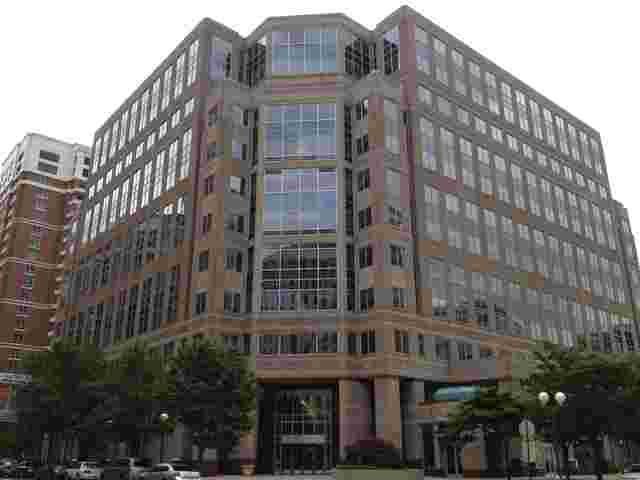
\includegraphics[width=2in]{ch-jpeg/nsf_hq_640x480-q10.jpg} & 
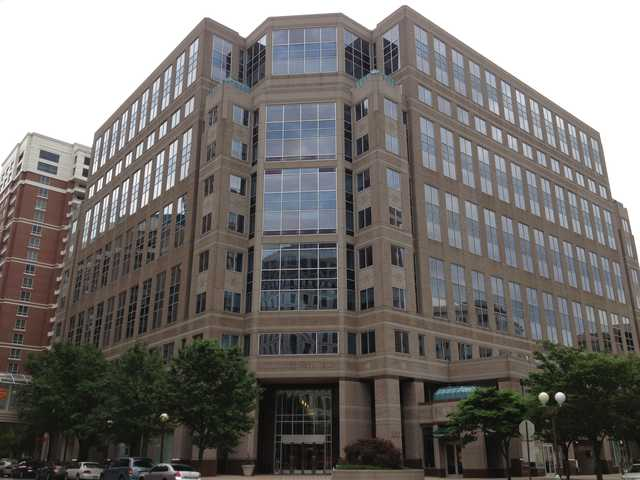
\includegraphics[width=2in]{ch-jpeg/nsf_hq_640x480-q50.jpg} &
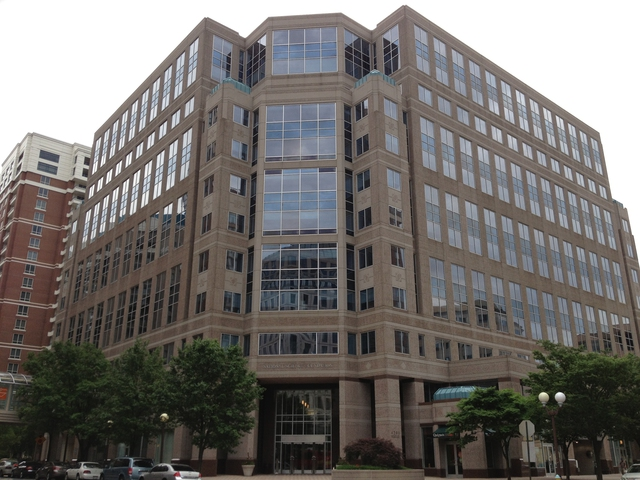
\includegraphics[width=2in]{ch-jpeg/nsf_hq_640x480-q99.jpg} \\
compression 10 & compression 50 & compression 99 \\
23,422 bytes & 49,305 bytes & 226,368 bytes \\
\end{tabular}
\caption{A test image showing three JPEG compression rates. Each image
  is 640x480 pixels. An uncompressed image would require 921,600 bytes.}
\end{figure}

The JPEG file itself is structured as a series of segments that are
concatenated together. Each segment has a specific kind of type; some
segments are fixed length, while others are variable. This kind of
format is sometimes called a ``chunk-based container file'' because
each segment can be thought of as a ``chunk'' and the file format is
designed to contain multiple distinct internal elements. The chunk
types are described in \tabref{tab:jpeg-format}.

Each JPEG chunk begins with the hex character |FF| followed by a code.
JPEG files are comprised of several segments that include a header, a
color table, a set of Huffman encoded data, and a footer, and may also
include icons and EXIF data (\figref{art/carving_jpeg}). 

\begin{table}
\begin{tabular}{lllll}
Code & Abbrev & Required? & Size & Meaning \\
\hline
FF D8 & \\
FF D9 & \\
\end{tabular}
\caption{JPEG chunk types}\label{tab:jpeg-format}
\end{table}
The JPEG standard describes specific chunk types. JPEG chunks 




\section{Thumbnails}

\section{Exif metadata}\label{sec:exif}
\subsection{GPS Coordinates}
\subsection{Date and Time}
\subsection{Other Exif Information}

\section{Non-obvious image content information}
\subsection{Non-Subject Information Leakage}
\subsection{Reflections}
\subsection{Details in Shadows}
\subsection{High-Resolution Information}


